%%%%%%%%%%%%%%%%%%%%%%%%%%%%%%%%%%%%%%%%%
% Developer CV
% LaTeX Template
% Version 1.0 (28/1/19)
%
% This template originates from:
% http://www.LaTeXTemplates.com
%
% Authors:
% Jan Vorisek (jan@vorisek.me)
% Based on a template by Jan Küster (info@jankuester.com)
% Modified for LaTeX Templates by Vel (vel@LaTeXTemplates.com)
%
% License:
% The MIT License (see included LICENSE file)
%
%%%%%%%%%%%%%%%%%%%%%%%%%%%%%%%%%%%%%%%%%

%----------------------------------------------------------------------------------------
%	PACKAGES AND OTHER DOCUMENT CONFIGURATIONS
%----------------------------------------------------------------------------------------

\documentclass[9pt]{developercv} % Default font size, values from 8-12pt are recommended

%----------------------------------------------------------------------------------------

\begin{document}

\def\photo{0}

%----------------------------------------------------------------------------------------
%	TITLE AND CONTACT INFORMATION
%----------------------------------------------------------------------------------------

\begin{minipage}[t]{0.41\textwidth} % 45% of the page width for name
	\vspace{-\baselineskip} % Required for vertically aligning minipages
	
	% If your name is very short, use just one of the lines below
	% If your name is very long, reduce the font size or make the minipage wider and reduce the others proportionately
	\colorbox{black}{{\HUGE\textcolor{white}{\textbf{\MakeUppercase{Edoardo}}}}} % First name
	
	\colorbox{black}{{\HUGE\textcolor{white}{\textbf{\MakeUppercase{Ghini}}}}} % Last name
	
	\vspace{6pt}
	
	{\huge Robotics and AI engineer} % Career or current job title
\end{minipage}
\hfill % Whitespace between
\begin{minipage}[t]{0.215\textwidth} % 27.5% of the page width for the second row of icons
	\vspace{-\baselineskip} % Required for vertically aligning minipages
        \if\photo1
          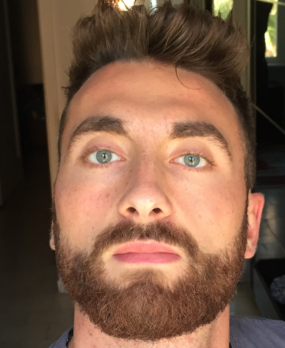
\includegraphics[width=0.75\textwidth]{meCropped}
        \fi
\end{minipage}
\hfill % Whitespace between
\begin{minipage}[t]{0.285\textwidth} % 27.5% of the page width for the first row of icons
	\vspace{-\baselineskip} % Required for vertically aligning minipages
	
	% The first parameter is the FontAwesome icon name, the second is the box size and the third is the text
	% Other icons can be found by referring to fontawesome.pdf (supplied with the template) and using the word after \fa in the command for the icon you want
        \icon{Phone}{12}{+33 6 73 03 31 71  (FR)}\\
	\icon{At}{12}{\href{mailto:ghiniedoardo@gmail.com}{ghiniedoardo@gmail.com}}\\	
	\icon{MapMarker}{12}{Nancy, France}\\
	\icon{Github}{12}{\href{https://github.com/dinies}{github.com/dinies}}\\
	\icon{LinkedinSquare}{12}{\href{https://www.linkedin.com/in/dinies/}{linkedin.com/in/dinies}}\\
\end{minipage}


\vspace{0.2cm}

%----------------------------------------------------------------------------------------
%	INTRODUCTION, SKILLS AND TECHNOLOGIES
%----------------------------------------------------------------------------------------

\begin{minipage}[t]{0.40\textwidth} % 40% of the page width for the introduction text
	\vspace{-\baselineskip} % Required for vertically aligning minipages
        \cvsect{Who am I?}\\
        Curious and self-confident person.\\
        Passionate about programming and believing it to be a form of art.\\
        Fascinated by mysteries of science and firm believer in technological progress.\\
        Enthusiastic about the latest academic discoveries in my field of expertise.\\
        Looking forward to learning more about Neuroscience and Human Consciousness and combine them together with Artificial Intelligence and Robotics.

     \vspace{0.1cm}

        \cvsect{Tools}\\
        \begin{center}
	  \bubbles{ 3/git, 5/Docker, 6/Cpp , 5/vim,  4/ROS,  3/unix}
        \end{center}

\end{minipage}
\hfill % Whitespace between
\begin{minipage}[t]{0.5\textwidth} % 50% of the page for the skills bar chart
	\vspace{-\baselineskip} % Required for vertically aligning minipages

        \cvsect{Theoretical Skills}
	\begin{barchart}{5.5}
		\baritem{Control theory}{50}
		\baritem{Robotic perception}{60}
		\baritem{Machine learning}{30}
		\baritem{Trajectory planning}{40}
		\baritem{Dynamic systems simulation}{50}
	\end{barchart}

        \vspace{0.5cm}
        \vspace{0.5cm}

        \cvsect{Programming Skills}
	\begin{barchart}{5.5}
	        \baritem{Algorithms design}{40}
	        \baritem{TDD}{50}
	        \baritem{OOP}{60}
	        \baritem{Containerization}{50}
	\end{barchart}

   \end{minipage}
%----------------------------------------------------------------------------------------
%	EXPERIENCE
%----------------------------------------------------------------------------------------

\vspace{0.5cm}

\cvsect{Experience}

\begin{entrylist}
        \entry
		{10/2020 -- 3/2022}
		{Robotics Engineer}
		{Inria , French national research institute for digital science and technology}
		{
                  Developed a system from the ground up to teleoperate an industrial robot in hazardous environments.
                }

        \entry
		{2/2019 -- 10/2019}
		{Master's Thesis}
		{La Sapienza, University of Rome}
		{
                Implemented a robotic system to achieve \textbf{autonomous navigation} (SLAM) in a urban environment of a mobile robot equipped with a \textbf{3D-LIDAR} laser sensors.\\
                The whole project has been implemented in C++ adopting the ROS build system.\\
                High-level features are extracted from the 3D-point cloud and categorized in geometric primitives.\\
                The sensor data is processed using the primitives in order to compute the trajectory of the robot.\\
                The work has been developed in collaboration with the university Robotics Lab.\\
                \href{https://github.com/dinies/MasterThesis-ArtificialIntelligence-Robotics/blob/master/MaterThesis_Edoardo_Ghini.pdf}{\textbf{Master thesis link}}\\
                }
	\entry
		{3/2016 -- 7/2016}
		{Back-end developer}
		{Translated}
                {
                  During this internship, I was responsible for the codebase of a web application:\textbf{Matecat}, written in PHP.\\
                  I developed unit-tests to certify the correctness of the core of the application.\\
                  Worked with databases and client-server communications: \textbf{MySQL} and \textbf{Apache}.\\
                  Brought code coverage percentage from 0\% to 25\%.\\
                  Learned how to work in \textbf{agile} teams, following \textbf{scrum} principles.\\
                  Acquired deep knowledge of advanced testing techniques: \textbf{Mock objects}, \textbf{Reflection}, and \textbf{TDD}.\\
                  \href{https://github.com/dinies/BachelorThesis/blob/master/EdoardoGhiniThesis.pdf}{\textbf{Bachelor thesis link}}\\
                }

\end{entrylist}

\newpage
%----------------------------------------------------------------------------------------
%	EDUCATION
%----------------------------------------------------------------------------------------

\cvsect{Education}

\begin{entrylist}
	\entry
		{2016 -- 2019}
		{Master's Degree - final grade 103/110}
		{La Sapienza, University of Rome}
		{Master in Artificial Intelligence and Robotics\\
                \texttt{Automation and Control}\slashsep
                \texttt{Mobile Robotics}\slashsep
                \texttt{Machine Learning}\slashsep
                \texttt{Neural Networks}
                }
	\entry
		{2013 -- 2016}
		{Bachelor's Degree - final grade 95/110}
		{Roma Tre University }
		{Computer Engineering \\
                \texttt{Operating Systems}\slashsep
                \texttt{Algorithms}\slashsep
                \texttt{Physics}\slashsep
                \texttt{Architectures}\slashsep
                \texttt{Software design}
                }
\end{entrylist}

\cvsect{Master's Degree thesis}


My Master Degree Thesis entailed the implementation of a mobile robotics SLAM system for \textbf{autonomous navigation} which performs 3D LIDAR Odometry and Tracking.\\
In particular the system extrapolates information about the \textbf{trajectory} of the robot carrying the laser sensor from the clouds of points that approximate the external environment.\\
The whole problem was solved using a probabilistic approach that involves using the \textbf{Gaussian assumption} and a \textbf{Least Square} formulation.\\
The entire project was developed in C++ using ROS and CMake and it had to address the compatibility with the robotics utility framework developed by the academic department.\\

\href{https://github.com/dinies/3D-Lidar-Odometry-and-Tracking}
{\textbf{3D-Lidar-Odometry GitHub Repository}}\\
\href{https://github.com/dinies/MasterThesis-ArtificialIntelligence-Robotics/blob/master/MaterThesis_Edoardo_Ghini.pdf }
{\textbf{Master's Degree thesis link}}\\

%----------------------------------------------------------------------------------------
%	ADDITIONAL INFORMATION
%----------------------------------------------------------------------------------------

\begin{minipage}[t]{0.3\textwidth}
	\vspace{-\baselineskip} % Required for vertically aligning minipages

	\cvsect{Languages}
	
	\textbf{Italian} - native\\
        \textbf{English} - IELTS academic cert.\\ Overall band score 7.0\\ CEFR level C1\\
\end{minipage}
\hfill
\begin{minipage}[t]{0.3\textwidth}
	\vspace{-\baselineskip} % Required for vertically aligning minipages
	
	\cvsect{Hobbies}

        I love sports:\\ Tennis, Basket, Football and  Chess.
        Keen reader of sci-finction novels.
	\end{minipage}
\hfill
\begin{minipage}[t]{0.3\textwidth}
	\vspace{-\baselineskip} % Required for vertically aligning minipages
	
	\cvsect{Other}

        Standard driving license, type B.\\
	Car owner.
\end{minipage}

\vspace{0.5cm}
\cvsect{Privacy}

"In compliance with the GDPR and Italian Legislative Decree no. 196 dated 30/06/2003, I hereby authorize the recipient of this document to use and process my personal details for the purpose of recruiting and selecting staff and I confirm to be informed of my rights in accordance to art. 7 of the above mentioned Decree".




%----------------------------------------------------------------------------------------

\end{document}
